\chapter{Evaluation}\label{chap:evaluation}
After developing a working prototype of the whole system, the next step was to prove that the solution satisfies the requirements.

This chapter describes the evaluation of the developed system.
In particular, the evaluation is divided into two parts:
\begin{enumerate}
    \item the first part involves the use of the developed system to solve a real-world problem;
    \item the second part is a qualitative evaluation of the developed visual language and development environment by users;
\end{enumerate}
As already mentioned, this twofold evaluation approach allows for assessing the user-friendliness of the development environment and the effectiveness of the visual language on one hand, and the expressivity and correctness of the latter on the other.

\section{Case Study}
In order for users to have a real-world problem to solve, both during the design phase with the focus group and during the evaluation phase with the end users, a use-case scenario was developed.

\subsection{Smart-Farming Scenario}

Since the \textit{IntellIoT} project already defines three sectors of application, namely \textit{Agriculture}, \textit{Healthcare} and \textit{Manufacturing}, the most natural choice was to use one of them to frame the case study.
The \textit{Agriculture} sector was chosen for multiple reasons.
First of all, it is probably the most familiar to the research group thanks to recent projects.
Moreover, it involves concepts that are easy to understand even for non-experts and it is possibly the most diverse.

Therefore, the case study was developed around the \textit{Smart Farming} scenario where the aim is to define an organization for a typical farm that adopts IoT technologies. Here is reported the text of the scenario:

\begin{quote}
Thanks to his investments, the farmer obtained the most cutting-edge technology machines to make his life easier.
After obtaining this technology, the farmer wants to organize the management of the daily chores of his ``smart farm'' by exploiting the machinery he possesses, which includes a self-driving tractor, multiple drones, an automatic irrigation system, and devices to take care of the animals.

With the acquired machinery, the farmer must irrigate the fields, which is highly demanding.
Therefore, the farmer purchased drones to improve the process of checking the soil and gathering information such as temperature and humidity, which the irrigator can use to calculate the amount of water needed.
The drones not employed for the former tasks will eliminate the moths and bugs that haunt the cultivation.

In addition, the farm always has a field that is currently not used to grow any crop.
However, the tractor must still plow the soil in that field.
To perform this function, it will need a set of waypoints.
The tractor can either have them computed by a drone flying over the field or as direct input from the farmer.

Finally, the farmer wants to harvest mature fruit and vegetables (we can assume that the tractor knows how to harvest).
After the harvest, the tractor can spray the field with pesticides to protect the crop.

As far as the animals are concerned, the farmer wants to feed them and have a daily health check-up for every animal. 
Moreover, he wants to collect the eggs from the hens and milk the cows and the goats.
It is worth mentioning that, during years of experience, the farmer noticed that feeding the animals before their health check-up makes them quieter, and the cows and the goats calmer when they get milked.
\end{quote}

\subsection{Use-Case Analysis}
Although not only one solution is possible for this example, here a reference one is described.
The approach to the problem, analogous to the one explicitly suggested to the focus group and to end users, consists of the following steps:
\begin{itemize}
    \item identify the roles of the organization;
    \item identify the groups of the organization;
    \item identify the tasks to be performed and possible relations between them;
    \item identify which roles are responsible for the tasks.
\end{itemize}
In particular, the approach used to solve the case study follows some simple guidelines.
As far as task decomposition is concerned, there could be different reasons why a task may be split into subtasks.
For instance, a task may be too complex to be performed by a single agent since it needs the capabilities of multiple agents.
Another reason may be that a task takes too much time to be performed atomically and it is better to split it into smaller tasks.
Moreover, a task may be decomposed into subtasks to use the achievement of a subtask as a precondition for the achievement of another task.
Finally, a task may be split into subtasks to allow for parallel execution of the subtasks by multiple agents.

On the other hand, when it comes to the definition of the roles, the approach mainly relies on the identification of a set of capabilities that the agent playing that role should provide in order to perform the tasks assigned to it.
For instance, referring to the ``write paper'' example in \cref{fig:moise-visual}, the role of the \texttt{writer} is defined by the capability of writing the sections of a paper, therefore agents playing that role can successfully perform the tasks regarding the writing of the section of the paper.

\subsubsection{Roles}
The approach to the problem starts by identifying the roles of the organization.
The ones defined for the case study are:
\begin{itemize}
    \item \textbf{Tractor Pilot} which will be played by agents that can drive a tractor.
    This role is abstract and can be specialized in:
    \begin{itemize}
        \item \textbf{Soil Plower}: played by an agent capable of plowing the soil;
        \item \textbf{Harvester}: played by an agent that can harvest the crops;
    \end{itemize}
    \item \textbf{Drone Pilot} which, in an analogous way to the tractor pilot, will be played by agents that can control a drone.
    Even this role is abstract and can be specialized in:
    \begin{itemize}
        \item \textbf{Temperature Checker}: played by an agent that can measure the temperature;
        \item \textbf{Humidity Checker}: played by an agent that can measure the humidity;
        \item \textbf{Bugs Eliminator}: played by an agent that can kill bugs;
    \end{itemize}
    \item \textbf{Irrigation System}: played by an agent that can irrigate the fields;
    \item \textbf{Animal Feeder}: played by an agent that can feed the animals;
    \item \textbf{Vet}: played by an agent that can perform a health check-up on the animals;
    \item \textbf{Product Collector}: played by agents that can collect the products from the animals.
    It is an abstract role that can be specialized in:
    \begin{itemize}
        \item \textbf{Egg Collector}: played by an agent that can collect the eggs from the hens;
        \item \textbf{Milk Collector}: played by an agent that can collect the milk from the cows and the goats;
    \end{itemize}
\end{itemize}

\subsubsection{Groups}
Once the roles are identified, the next step is to identify the groups of the organization.
In particular, the groups are defined as follows:
\begin{itemize}
    \item \textbf{Farm Group}: it is a group of agents that can perform the tasks related to the farm.
    In this scenario, there are no roles that directly belong to this group.
    However, it contains the following subgroups:
    \begin{itemize}
        \item \textbf{Field Group}: a group of agents that can perform the tasks related to the fields.
        The roles that belong to this group are: \textit{Soil Plower}, \textit{Harvester}, \textit{Temperature Checker}, \textit{Humidity Checker}, \textit{Bugs Eliminator}, and \textit{Irrigation System};
        \item \textbf{Animal Group}: a group of agents that can perform the tasks related to the animals.
        The roles that belong to this group are \textit{Animal Feeder}, \textit{Vet}, \textit{Egg Collector}, and \textit{Milk Collector}.
    \end{itemize}
\end{itemize}

\subsubsection{Tasks/Goals}
The next step involves identifying the tasks, or goals, to be performed and the possible relations between them.

The first goal encountered is \textit{Irrigate Field}.
However, the latter needs some intermediate steps to be achieved and, therefore, it has dependencies on other goals.
In particular, the \textit{Calculate Water} is needed so that the irrigator knows how much water to use.
In turn, the \textit{Calculate Water} goal needs the \textit{Measure Temperature} \textbf{and} \textit{Measure Humidity} goals to be achieved.

Proceeding with the scenario, the next goal is \textit{Eliminate Bugs}.
The \textit{Eliminate Moths} goal could be also identified, but, for simplicity, it is not considered.

The next goal is \textit{Plough Field} that needs either the \textit{Compute Waypoints} or the \textit{Input Waypoints} goals to be achieved, therefore it depends on them with an \textbf{or} relation.

Next, the \textit{Harvest} goal is identified, which also enables the \textit{Spray Pesticides} goal.

Finally, the goals concerning the animals are defined.
In particular, the \textit{Feed Animals}, \textit{Health Check-Up}, and \textit{Collect Products} goals are identified.
The latter can be further specialized in \textit{Collect Eggs} and \textit{Collect Milk}.
In turn, \textit{Collect Milk} needs the \textit{Milk Cows} and \textit{Milk Goats} goals to be achieved.
Moreover, the \textit{Feed Animals} goal enables all the other goals related to the animals.

As far as the assignation of the goals to the roles is concerned, \cref{tab:goal-assignation} shows the result of the analysis:

\begin{table}[H]
    \centering
    \begin{tabular}{| l | l |}
        \hline
        \textbf{Goal} & \textbf{Responsible Role} \\
        \hline
        Irrigate Field & Irrigation System \\
        Calculate Water & Irrigation System \\
        Measure Temperature & Temperature Checker \\
        Measure Humidity & Humidity Checker \\
        Eliminate Bugs & Bugs Eliminator \\
        Plough Field & Soil Plower \\
        Compute Waypoints & Drone Pilot \\
        Harvest & Harvester \\
        Spray Pesticides & Tractor Pilot \\
        Feed Animals & Animal Feeder \\
        Health Check-Up & Vet \\
        Collect Products & Product Collector \\
        Collect Eggs & Egg Collector \\
        Collect Milk & Milk Collector \\
        Milk Cows & Milk Collector \\
        Milk Goats & Milk Collector \\
        \hline
    \end{tabular}
    \caption{Assignation of the goals to the responsible roles.}
    \label{tab:goal-assignation}
\end{table}

\section{Solution with the Visual Language}
In this section, a solution for the above scenario using the developed visual language is presented.

\begin{figure}[H]
    \centering
    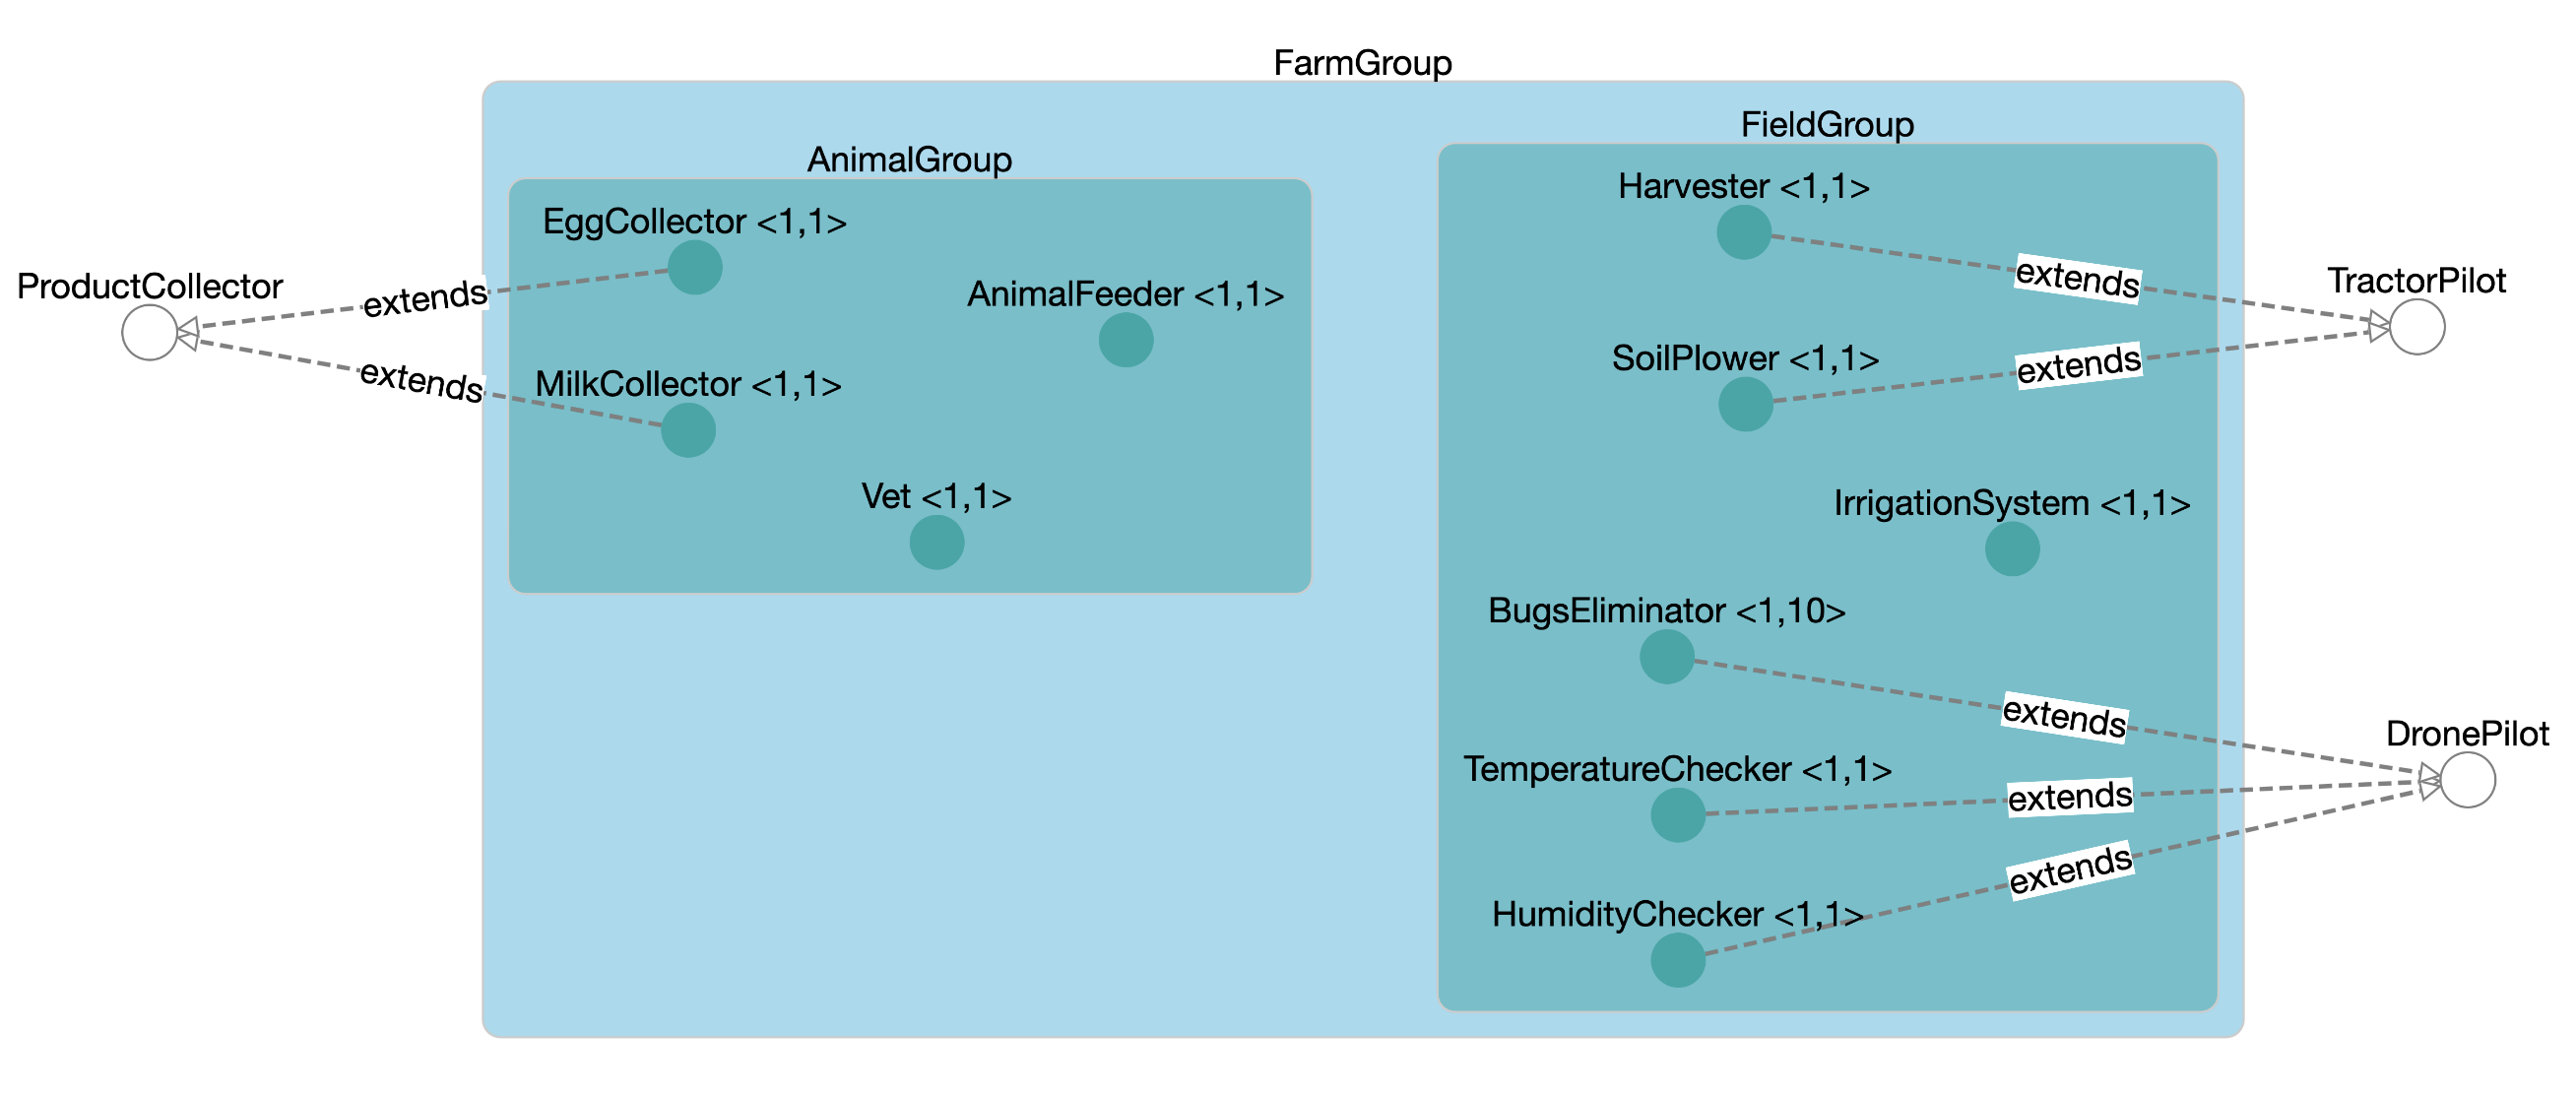
\includegraphics[width=\textwidth]{images/solution-structural.png}
    \caption{Solution for the structure of the organization.}
    \label{fig:solution-structural}
\end{figure}

In \cref{fig:solution-structural} the solution regarding the structure of the organization is presented.
The outermost rectangle represents the \texttt{Farm Group} that contains two subgroups, \texttt{Animal Group} and \texttt{Field Group}, depicted by the two inner rectangles.
The three circles that are not placed inside any group represent the abstract roles \texttt{Product Collector}, \texttt{Tractor Pilot}, and \texttt{Drone Pilot}.
As for the other roles, they are concrete and therefore placed inside their corresponding group.
Some of them extend the abstract roles, as is the case of \texttt{Egg Collector} and \texttt{Milk Collector} that extend \texttt{Product Collector}.
Finally, the cardinality of the roles inside the groups is represented in the form \texttt{\textless min,max\textgreater}.
For instance, the \texttt{Bugs Eliminator} role has to be played by at least 1 agent and at most 10 agents while all the other roles have to be played by exactly 1 agent.

\begin{figure}[H]
    \centering
    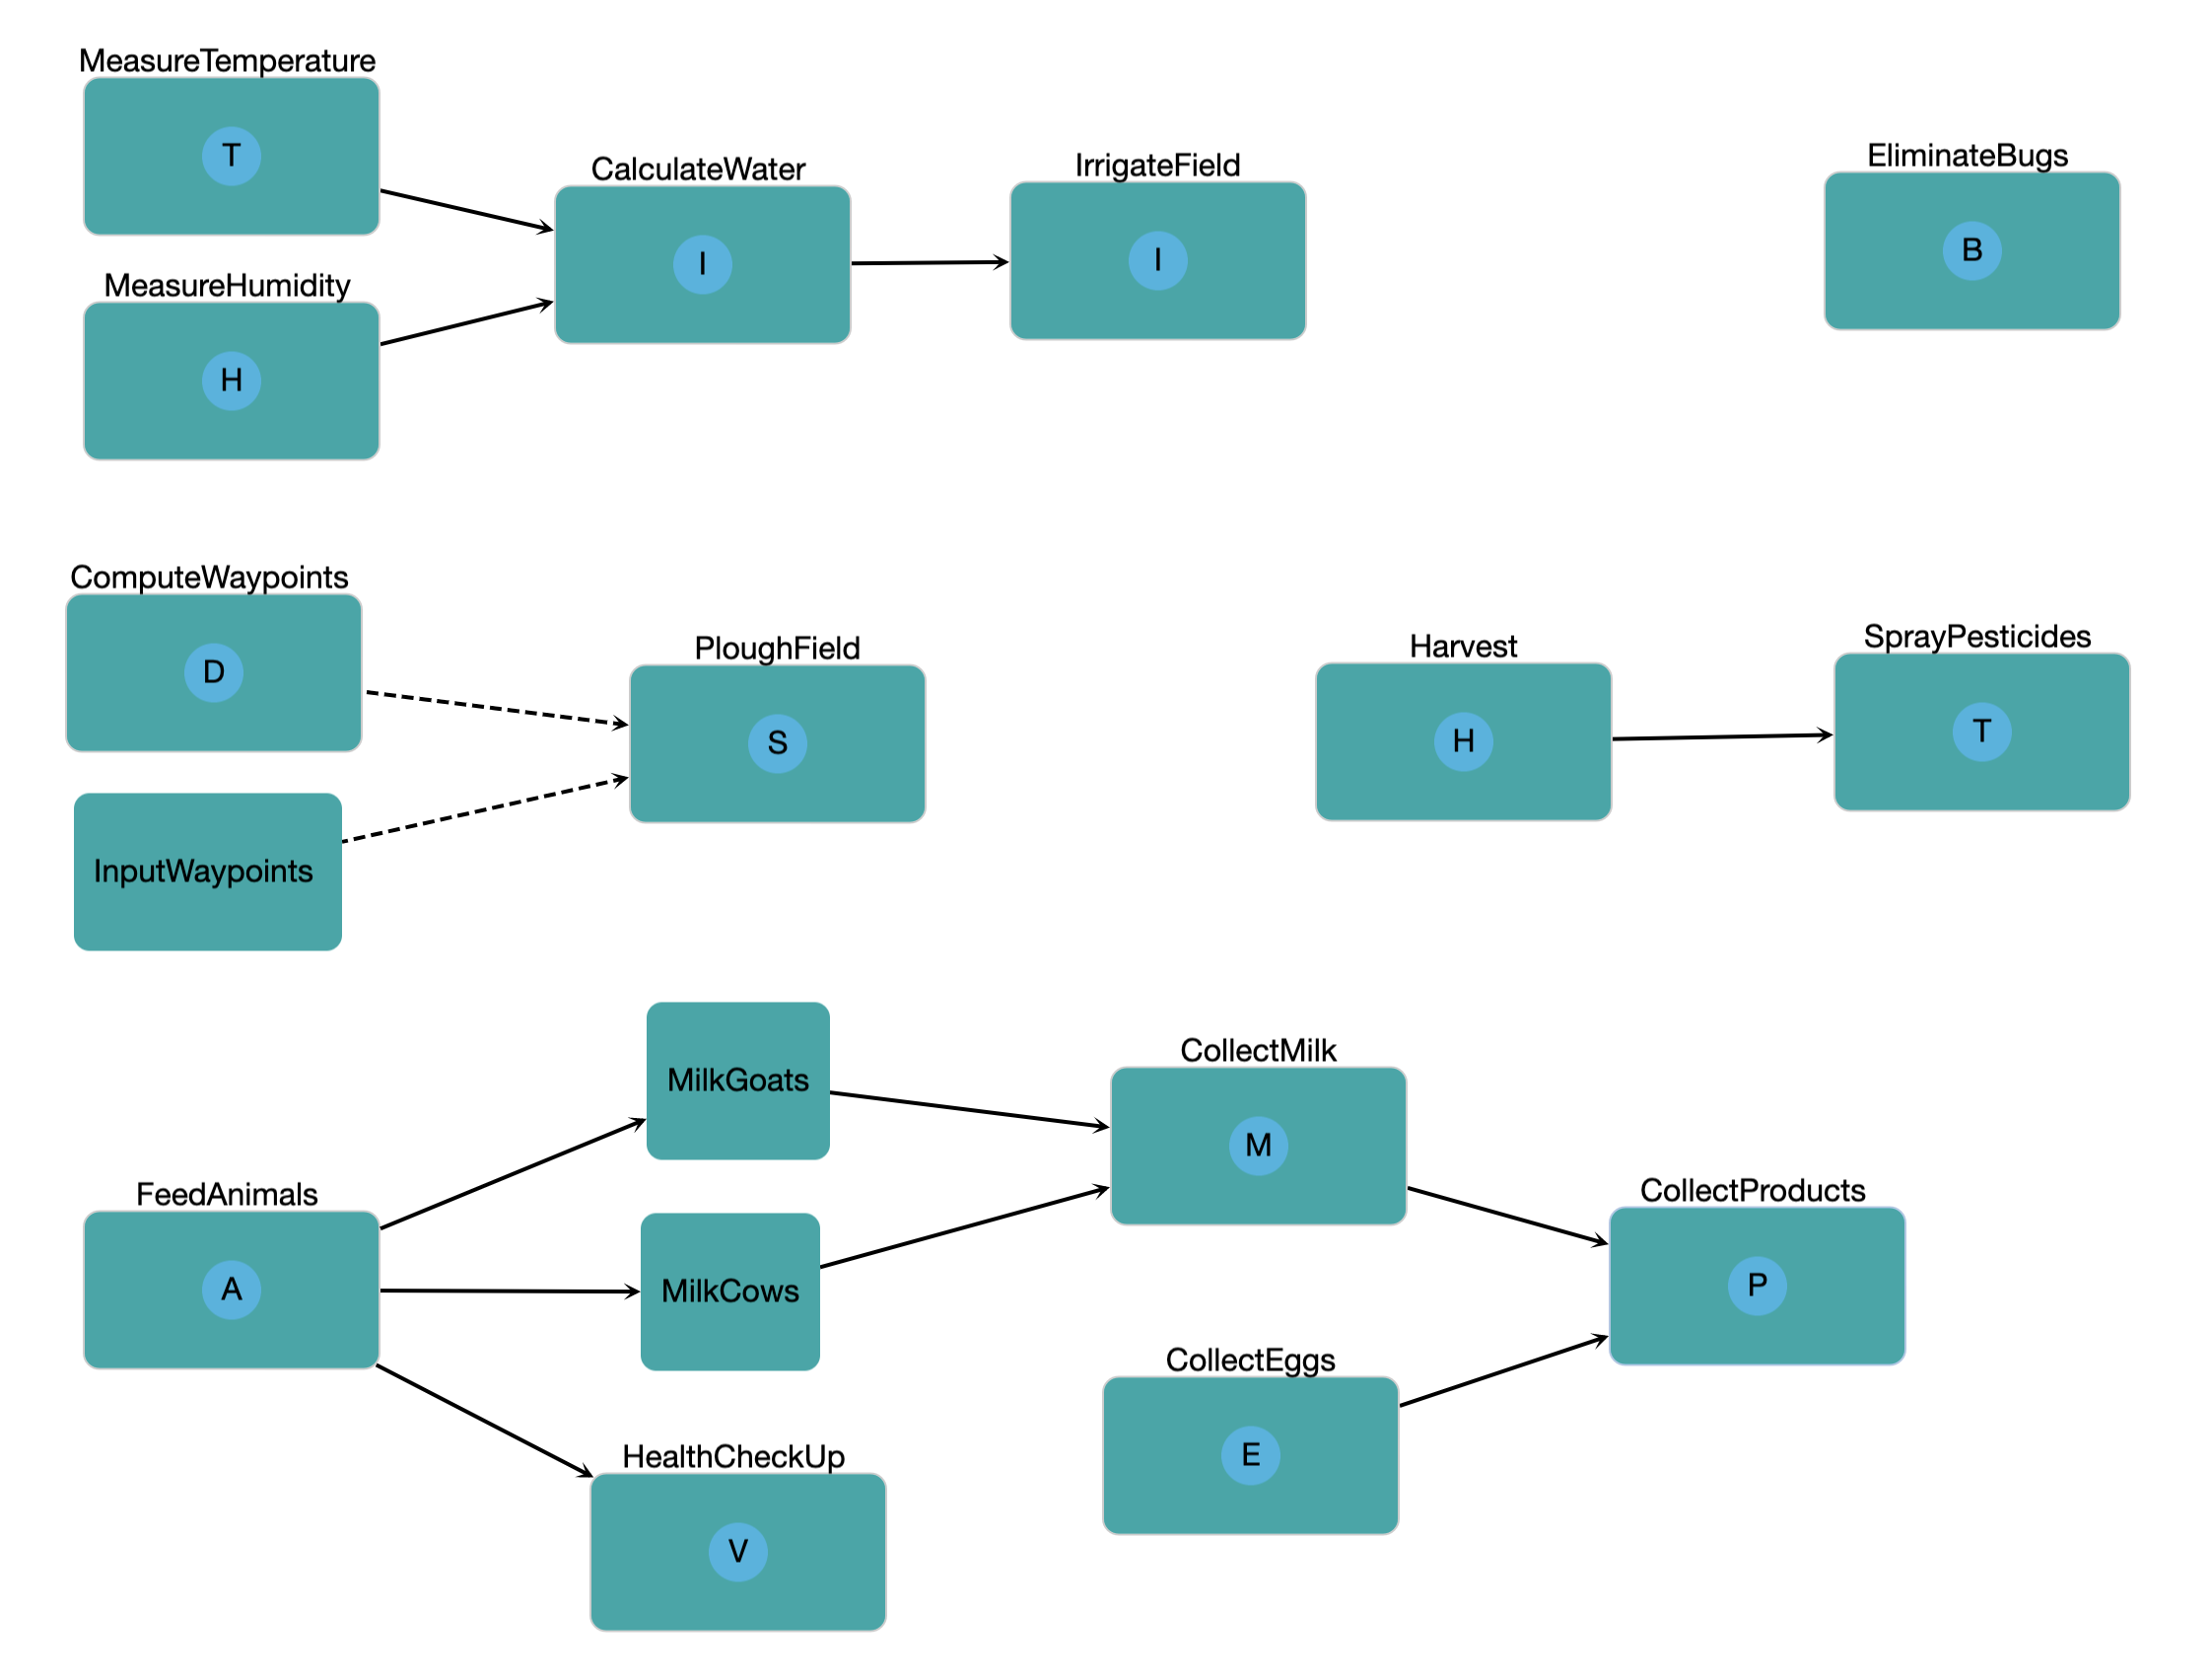
\includegraphics[width=\textwidth]{images/solution-functional.png}
    \caption{Solution for the behavior of the organization.}
    \label{fig:solution-functional}
\end{figure}

As far as the behavior of the organization is concerned, \cref{fig:solution-functional} shows its solution with the visual language.
For instance, the \texttt{Collect Products} goal requires the \texttt{Collect Milk} and \texttt{Collect Eggs} goals to be achieved, therefore, it depends on them with an \textbf{and} relation.
The latter is represented by the solid arrows that connect the enabler goals to the enabled goal.
Indeed, the use of dashed arrows would indicate an \textbf{or} relation, like the one between the \texttt{Compute Waypoints} and \texttt{Input Waypoints} goals and the \texttt{Plough Field} goal.
In turn, the \texttt{Collect Milk} goal requires the \texttt{Milk Cows} and \texttt{Milk Goats} goals to be achieved.
Again, the former depends on the latter goals with an \textbf{and} relation.
Moreover, the \texttt{Milk Cows} and \texttt{Milk Goats} goals need the \texttt{Feed Animals} goals to be achieved in order for them to be pursued.
Finally, the latter goal also enables the \texttt{Health Check-Up} goal.

To conclude, the assignation of the goals to the roles is represented by the presence of the circle corresponding to the role inside the rectangle representing the goal.
For instance, the \texttt{Vet} is responsible for the \texttt{Health Check-Up} goal.

\section{Users' Test}
Due to the shortage of time, it was nearly impossible to gather a large number of users to test the developed visual language.
Moreover, even though the target users for the system are domain experts, finding them and having them test the system would not have been feasible.

Thus, the users' test was performed on a small number of people from the research group.
Since the users have a background in computer science and some of them are familiar with the domain of the scenario, the result was expected to be slightly optimistic but still useful to evaluate the usability of the system.

\subsection{Test Description}
The test consisted in asking the users to provide a solution for the smart-farming scenario using the Web IDE and therefore exploiting the designed visual language.
The vast majority of the users were already familiar with the scenario since they participated in the focus group sessions that helped the design of the visual language itself.
They were also asked to think aloud while they were building the solution, so that possible doubts could be clarified, mainly about the meaning of the concepts of the organization model such as roles, groups, and goals.

After the users had provided their solutions, they were asked to provide feedback through a short questionnaire.
The latter was composed of a few questions about every step of the process, from the identification of the core concepts of the organizations to the use of the Web IDE to build the solution.

The questions were designed to evaluate the usability of the system and the visual language on one hand, and the effectiveness of the organization model on the other, that is the ability of the model to represent the organization in a way that is natural and understandable for the users.
Specifically, the questions were modeled as statements such as \textit{It was easy for me to identify what roles are needed in the organization} and \textit{It was easy for me to create the roles using the IDE}.

The participants were asked to rate the statements on a scale from $1$ to $5$, where $1$ means that they strongly disagreed with the statement and $5$ means that they strongly agreed with the statement.

\subsection{Results}
Even though some of the users needed some hints to get started, all of them were able to provide a solution for the scenario in an acceptable amount of time, with the average time being around $25$ minutes.

All the solutions provided by the users produce a syntactically correct organization specification, which means that no errors will be encountered when the system tries to deploy the organization.
However, the solutions provided by the users are not all necessarily semantically correct, that is, they might not represent the organization in a way that completely matches and satisfies the requirements of the scenario.

What the users most struggled with was the identification of the roles and the groups.
Specifically, they had difficulties in distinguishing the concepts of agents and the roles played by them.
Moreover, some of them had difficulty understanding that roles have to be inserted in groups.
On the other hand, the users easily understood the concept of goals and were able to identify them in the scenario together with the relations between them.

However, once the users were explained the meaning of the concepts and some fundamentals of the organization model, they were able to provide a solution for the scenario in a short amount of time.

As far as the use of the Web IDE is concerned, all the users had no issues in creating the visual components and interacting with them.
What is more, the navigation through the different pages of the IDE was straightforward for all the users.

Therefore, these results show that the visual language is intuitive and that the Web IDE is easy to use.
As far as the organization model is concerned, it appears to be effective in representing the organization powerfully and flexibly, even though some of the users do not inherently reason about organizations in terms of the model's concepts.
Nevertheless, it turned out to be simple enough to be easily understood by the users when they are briefly introduced to the main concepts.

In \cref{fig:questionnaire-results-model} and \cref{fig:questionnaire-results-ui} the ratings of the statements are shown.
The first figure shows the results for the statements related to the organization model, that is the identification of the core concepts of the organization.
On the other hand, the second figure shows the results for the statements related to the use of the Web IDE.
Each color represents a step of the process of the test, that is, the identification and creation of the roles, groups, goals, dependencies among goals, and the assignation of goals to roles, respectively.

According to the feedback provided by the users, the result of the test is extremely positive.
As already stated, the results were expected to be slightly optimistic since the users are familiar with the domain and the organization model.
However, the results show that the organization model is effective in representing the organization and that the visual language is intuitive and easy to use.

Finally, it is worth noting that the user that provided the most complete solution for the scenario was a computer science student that had never heard of MAS organizations before, proving that there is no need for a specific background and previous experience to define one.

\begin{center}
    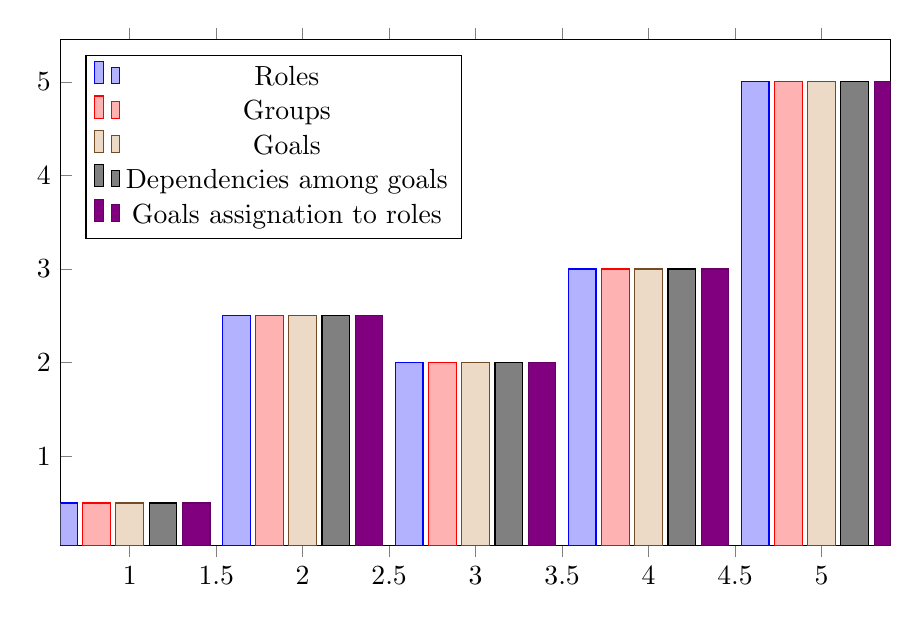
\begin{tikzpicture}
    \begin{axis} [ybar,width=\linewidth,height=8cm,legend pos=north west]
    \addplot coordinates {
        (1,0.5) 
        (2,2.5) 
        (3,2) 
        (4,3)
        (5,5)
    };
    \addplot coordinates {
        (1,0.5) 
        (2,2.5) 
        (3,2) 
        (4,3)
        (5,5)
    };
    \addplot coordinates {
        (1,0.5) 
        (2,2.5) 
        (3,2) 
        (4,3)
        (5,5)
    };
    \addplot coordinates {
        (1,0.5) 
        (2,2.5) 
        (3,2) 
        (4,3)
        (5,5)
    };
    \addplot coordinates {
        (1,0.5) 
        (2,2.5) 
        (3,2) 
        (4,3)
        (5,5)
    };
    \legend {Roles, Groups, Goals, Dependencies among goals, Goals assignation to roles};
    \end{axis}
    \end{tikzpicture}
    \captionof{figure}{Average rating of the statements concerning the identification of the main concepts of the organization model.}
    \label{fig:questionnaire-results-model}
\end{center}

\begin{center}
    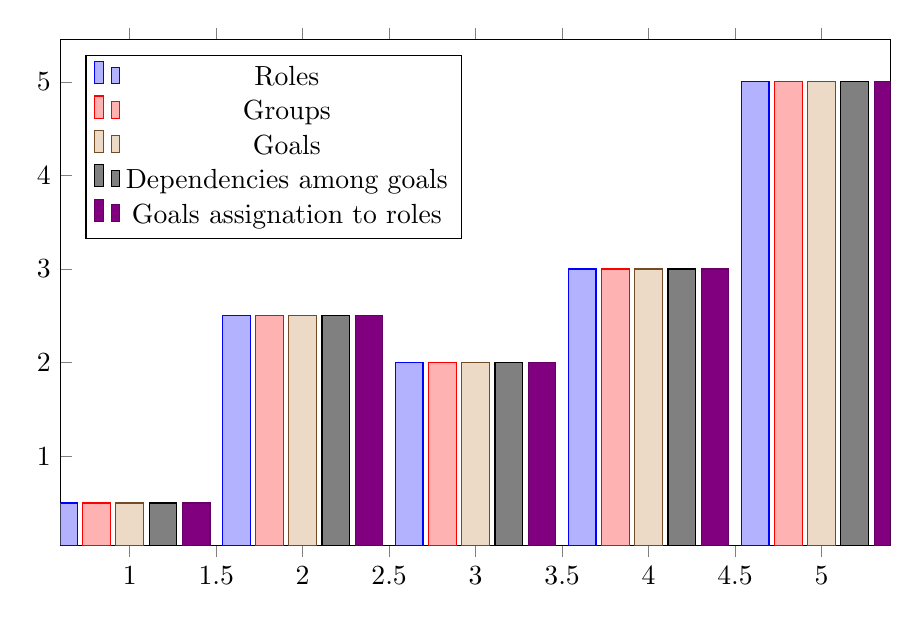
\begin{tikzpicture}
    \begin{axis} [ybar,width=\linewidth,height=8cm,legend pos=north west]
    \addplot coordinates {
        (1,0.5) 
        (2,2.5) 
        (3,2) 
        (4,3)
        (5,5)
    };
    \addplot coordinates {
        (1,0.5) 
        (2,2.5) 
        (3,2) 
        (4,3)
        (5,5)
    };
    \addplot coordinates {
        (1,0.5) 
        (2,2.5) 
        (3,2) 
        (4,3)
        (5,5)
    };
    \addplot coordinates {
        (1,0.5) 
        (2,2.5) 
        (3,2) 
        (4,3)
        (5,5)
    };
    \addplot coordinates {
        (1,0.5) 
        (2,2.5) 
        (3,2) 
        (4,3)
        (5,5)
    };
    \legend {Roles, Groups, Goals, Dependencies among goals, Goals assignation to roles};
    \end{axis}
    \end{tikzpicture}
    \captionof{figure}{Average rating of the statements concerning the ease of use of the Web IDE when defining the concepts.}
    \label{fig:questionnaire-results-ui}
\end{center}

